\chapter{Implementation}
\label{ch:implementation}
In this chapter we will discuss several implementation details that
is important for understanding the work. We will also show
the code patterns examples that were mentioned in the \autoref{sec:quality_concerns}.

\section{TensorFlow}
In the figure \ref{fig:model_uml}, you might notice that some of the functions
return \lstinline{tf.Tensor} object. In order to understand what it is,
let's make a small example to show how a TensorFlow program can look.
In the listing \ref{list:tf_graph}, you can find a small TensorFlow program.



\begin{lstlisting}[language=Python, caption={TensorFlow example (source: \cite{tensorflow2015-whitepaper)}},label={list:tf_graph}]
import tensorflow as tf
b = tf.Variable(tf.zeros([100])) # 100-d vector, init to zeroes
W = tf.Variable(tf.random_uniform([784,100],-1,1)) # 784x100 matrix w/rnd vals
x = tf.placeholder(name="x") # Placeholder for input
relu = tf.nn.relu(tf.matmul(W, x) + b) # Relu(Wx+b)
C = [...] # Cost computed as a function
# of Relu
s = tf.Session()
for step in xrange(0, 10):
	input = ...construct 100-D input array ... # Create 100-d vector for input
	result = s.run(C, feed_dict={x: input}) # Fetch cost, feeding x=input
	print step, result
\end{lstlisting}


In TensorFlow, computations are represented as a directed graph that is composed
of nodes. The computational graph of the listing \ref{list:tf_graph}, is shown
in the figure \ref{fig:comp_graph_tf}. Values that flow along the graph are denoted
as \emph{Tensor}, which is a TensorFlow representation of primitive values shaped
into an array. Another important concept in TensorFlow is an operation, which represent
an abstract computation. For example, in figure \ref{fig:comp_graph_tf} you can see
such operations: 'ReLU', 'Add', 'MatMul'.


\begin{figure}[H]
	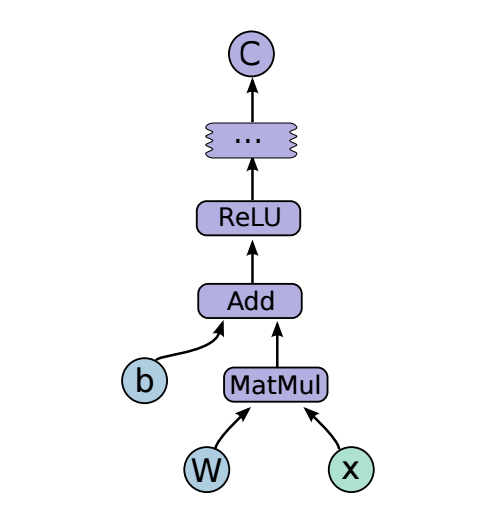
\includegraphics[width=\linewidth]{comp_graph_tf}
	\caption{Computational graph of the listing \ref{list:tf_graph} (source: \cite{tensorflow2015-whitepaper})}
	\label{fig:comp_graph_tf}
\end{figure}


To execute a TensorFlow program, one needs to build the computational graph,
and then execute it. We're building
the computation graph by instantiating the TensorFlow classes like the
\lstinline{tf.Variable}. But to actually compute this and obtain the correct output values
we need to execute this using the \lstinline{tf.Session}. The \lstinline{tf.Session}
is
responsible for the execution of the computational graph; it takes the graph
as well as the data
to execute it on desired environment(e.g. GPU, CPU). One also passes the parameter
\lstinline{feed_dict} that is a dictionary object where the key has the name of
\lstinline{tf.placeholder} and the value is the data that the placeholder should be substituted
with. A \emph{placeholder} is a promise to provide the value later in the program.


% \paragraph{How the computation works in tensorflow, sessions}
% \paragraph{How the data coming in --> Placeholders}
%
% \paragraph{what is tensor}
% \paragraph{what is ops}

\section{Code quality}
In the \autoref{sec:quality_concerns}, we talked about quality concerns
that need be taken into account to improve the quality of the prototype.
These recommendation were carefully followed in the implementation of this work.

\subsection{Code patterns in the code} We introduced code patterns in the
\autoref{sec:quality_concerns}, that are
helpful for understanding and reasoning about the code. Here we will show
examples of how this code patterns was applied in the prototype.

\subparagraph{Method comment} Would be perfect, if the code would
be so clear and readable that we could avoid unnecessary comments in it.
The method comment can help with this. Instead of having a comment in the code,
it encourages to write a function with self-explanatory name:
\begin{lstlisting}[language=Python, caption={Method comment example},label={list:method_comment}]
def init_location_network(config):
    """Initialise location network using `loc_net` scope and return it."""
    with tf.variable_scope('loc_net'):
        loc_net = LocNet(config)
    return loc_net
\end{lstlisting}

We could put this code  with an explanation
comment directly in the place where this function is called, but having
a function with the name \lstinline{init_location_network} should be more than enough
to understand that the function is initializing the location network.

\subparagraph{Composed method} This encourages function to have an identifiable
task and that all operations performed in the function should be on the same
level of abstraction.

\begin{lstlisting}[language=Python, caption={Method comment example},label={list:composed}]
def init_seq_rnn(images_ph, labels_ph):
    """Feed locations to LSTM cells and return output of LSTM cells."""
    # Core network.
    N = tf.shape(images_ph)[0]
    glimpse_net = init_glimpse_network(images_ph)
    loc_net = init_location_network(Config)
    pick_net = init_picker_network(Config)
    inputs = lstm_inputs(glimpse_net, N)
    lstm_cell, init_state = init_lstm_cell(Config, N)

    def get_next_input(output, i):
        loc, loc_mean = loc_net(output)
        n_image = pick_net(output)
        gl_next = glimpse_net(loc, n_image)
        loc_mean_arr.append(loc_mean)
        sampled_loc_arr.append(loc)
        return gl_next

    outputs, _ = seq2seq.rnn_decoder(
        inputs, init_state, lstm_cell, loop_function=get_next_input
    )
    return outputs
\end{lstlisting}

In the listing \ref{list:composed}, you can see the example of the composed method.
As you might guess from the function name \lstinline{init_seq_rnn}, the
function
is initialising the sequence of \gls{RNN} cells, which is indeed an identifiable task.
Additionally, all of the operations performed in the function
have a high level of abstraction: for example to
create \gls{LSTM} inputs or to initialise glimpse network, it uses helper functions
\lstinline{lstm_inputs} and \lstinline{init_glimpse_network} respectively.
For the understanding the composed method, one can skip the function \lstinline{get_next_input}.

\subparagraph{Temporary variable} This pattern recommends using a temporary
variable with self-explanatory name instead of having very long expression
in the code. One of the example of this pattern you can see
in the listing \ref{list:comment_method}.

\begin{lstlisting}[language=Python, caption={Method comment example},label={list:comment_method}]
img_size = (
	Config.original_size * Config.original_size * Config.num_channels
)
images_shape = [None, Config.n_img_group, img_size]
labels_shape = [None, Config.n_img_group]
with tf.variable_scope('data'):
	images_ph = tf.placeholder(tf.float32, images_shape, name='images')
	labels_ph = tf.placeholder(tf.int64, labels_shape, name='labels')
\end{lstlisting}

The variables \lstinline{img_size}, \lstinline{images_shape}, \lstinline{labels_shape}.
increase readability by avoiding very long expressions in the lines after.
The names make it also easier to comprehend for those who are unfamiliar
with the code.

\subparagraph{Duck typing} This a concept that is used by dynamic typed languages.
The idea behind it is that to use an object, it has to have a certain desired functionality,
but it does not matter the nature of this object.
\begin{lstlisting}[language=Python, caption={Method comment example},label={list:duck_typing}]
if(not(hasattr(dataset, "labels") and hasattr(dataset, "images"))):
	raise ValueError(
		'dataset object should have properties: `images` and `labels`'
	)
\end{lstlisting}

In the listing \ref{list:duck_typing}, you can see a clear example of duck typing.
It's important that the object \lstinline{dataset} is having properties
\lstinline{images} and \lstinline{labels}, but we don't care about it's nature,
i.e. what class the object \lstinline{dataset} is instantiated from.

\paragraph{Code conventions} The current implementation follows the
docstring conventions described in guide PEP 257 \cite{Goodger2001}, as it was
suggested in \autoref{sec:quality_concerns}. The convention for code layout,
indentation and names of functions, classes and variables is consistent with
the guide PEP 008 \cite{Rossum}. To stay consistent with best and common practices
in python, the current implementation relies on the
"The Hitchhiker’s Guide to Python"\footnote{\cite{Reitz}}. It gives us
the conventions of how to configure, structure, test and document the code.
% \paragraph{Naming, Code readability}

\section{Implementation details}
The purpose of this section is to show the implementation details that
are important to understand the code and the model.

\paragraph{Hybrid loss} One of the essential aspect in machine learning is to
define the loss function carefully.
In this work, we have reinforcement learning aspects as a part of the training,
therefore our loss function is composed
of multiple loss function:
\begin{itemize}
	\item loss function to train the location network with
		help of reinforcement learning algorithms by increasing rewards.
	\item loss function to train the baseline function that is used to
		reduce the variance when computing the gradient of loss function for
		the location and picker networks.
	\item loss function to train the classification network based on the ground truth.
\end{itemize}


You can see the way it's computed in listing \ref{list:hybrid_loss}}

\begin{lstlisting}[language=Python, caption={Hybrid loss},label={list:hybrid_loss}]
baselines = init_baseline_net(outputs)

logits = inference(outputs[-1])
softmax = tf.nn.softmax(logits)

xent = cross_entropy_with_logits(logits, labels_ph)

pred_labels = tf.argmax(logits, 1)

rewards = get_rewards(pred_labels, labels_ph)

logll = loglikelihood(loc_mean_arr, sampled_loc_arr, Config.loc_std)

advs = rewards - tf.stop_gradient(baselines)
logllratio = tf.reduce_mean(logll * advs)

baselines_mse = tf.reduce_mean(tf.square((rewards - baselines)))
var_list = tf.trainable_variables()
# hybrid loss
loss = -logllratio + xent + baselines_mse  # `-` for minimize
\end{lstlisting}

where \lstinline{outputs} - are the output from \gls{LSTM} cell,
\lstinline{xent} - is the cross entropy between predicted values and ground truth,
\lstinline{baselines_mse} - is the mean squared error loss between actual rewards
and expected reward(baseline),
\lstinline{logllratio} - is the loss for the location network, which is trained
using REINFORCE rule which was described in \autoref{ss:pol_based_rl}.

\paragraph{Gradient computation} Normally, users of TensorFlow train the model
by calling \lstinline{minimize} function from an optimizer: \lstinline{Optimizer.minimize(loss)}
However, since in our case we clip the gradient values
to prevent the vanishing and the exploding gradient problems, we firstly
need to compute gradients, then clip the values, and apply gradients:

\begin{lstlisting}[language=Python, caption={gradient computation},label={list:comp_grad}]
grads = tf.gradients(loss, var_list) # computes gradients with respect to var_list
clipped_grads, _ = tf.clip_by_global_norm(grads, Config.max_grad_norm) # clip the values
optimizer = tf.train.AdamOptimizer(learning_rate) # Initialise the optimizer
train_op = optimizer.apply_gradients(
	zip(clipped_grads, var_list), global_step=global_step
) # apply the capped gradients
\end{lstlisting}
where \lstinline{var_list} - is the variables with respect to which the gradient should
be computed.

We get the \lstinline{var_list} by using TensorFlow function \lstinline{tf.trainable_variables()},
which return all of the trainable variables in the graph. One thing to notice is
that for some variables like location or baselines we use function \lstinline{tf.stop_gradient},
these prevent the contribution of the variable to be taken into account when computing a
gradient. The function \lstinline{tf.trainable_variables()} returns the trainable variables excluding
the variables where the function \lstinline{tf.stop_gradient} was applied on.
